\label{testes}
\chapter{TESTES}

O presente capítulo tem como objetivo descrever quais foram os testes realizados durante o desenvolvimento do projeto Vocco a fim de garantir um controle de qualidade preciso da aplicação.

\section{Plano de testes}
 Nesta seção, será detalhado o modo como serão realizados os testes do sistema. Assim garantindo que as funções principais estejam de acordo com os requisitos propostos.

 \subsection{Teste de funcionalidade de Instituição}
 
\begin{itemize}
    \item \textbf{Cenário Ideal Cadastro de Instituição:}
Descrição do cenário ideal de usabilidade do usuário no processo de cadastro de instituição.
    
\begin{figure}[ht]
        \centering
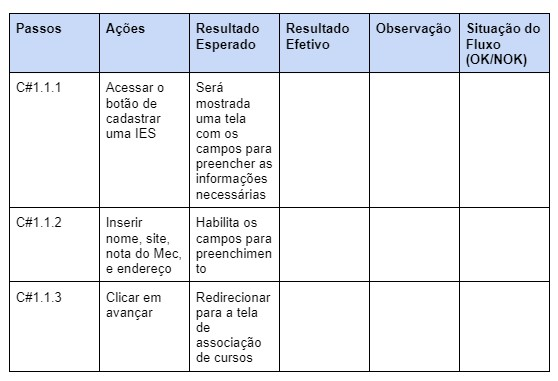
\includegraphics[width=0.80\textwidth]{images/teste-cad-instituicao-feliz.jpg}
        \caption{Cenário ideal cadastro de instituição}
        \label{commitsAturo}
    \end{figure}
O processo ideal de cadastro de instituição percorre três ações para ser concluído.

\newpage
    
    \item \textbf{Cenário de Exceção Cadastro de Instituição:}
Descrição do cenário de exceções de usabilidade do usuário no processo de cadastro de instituição.

\begin{figure}[ht]
        \centering
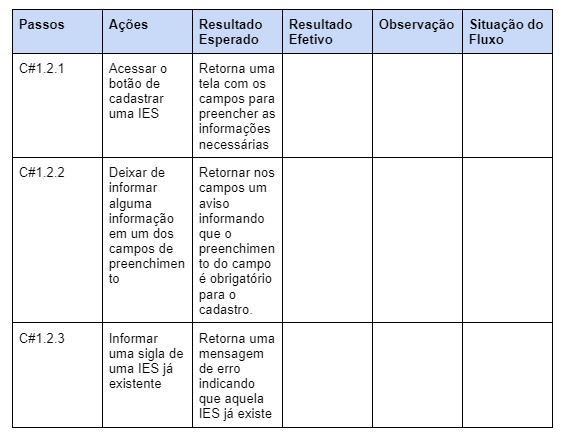
\includegraphics[width=0.80\textwidth]{images/teste-cad-instituicao-excecao.jpg}
        \caption{Cenário de exceção de cadastro de instituição}
        \label{commitsAturo}
    \end{figure}

O processo com exceções de cadastro de instituição percorre três ações para ser concluído.

\newpage
    
     \item \textbf{Cenário Ideal Listagem de Instituição:}
Descrição do cenário ideal de usabilidade do usuário no processo de listagem de instituição.

\begin{figure}[ht]
        \centering
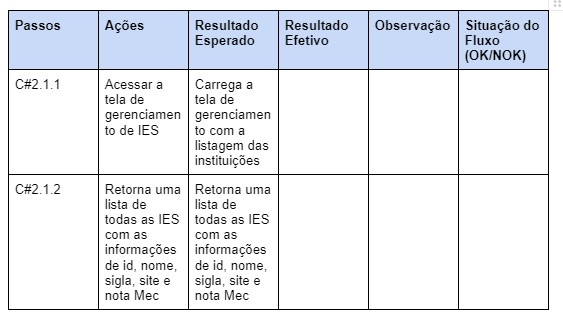
\includegraphics[width=0.80\textwidth]{images/teste-list-instituicao-feliz.jpg}
        \caption{Cenário ideal de Listagem de instituição}
        \label{commitsAturo}
    \end{figure}

O processo ideal de listagem de instituição percorre duas ações para ser concluído.


    \item \textbf{Cenário de Exceção Listagem de instituição:}
Descrição do cenário de exceções de usabilidade do usuário no processo de listagem de instituição.

\begin{figure}[ht]
        \centering
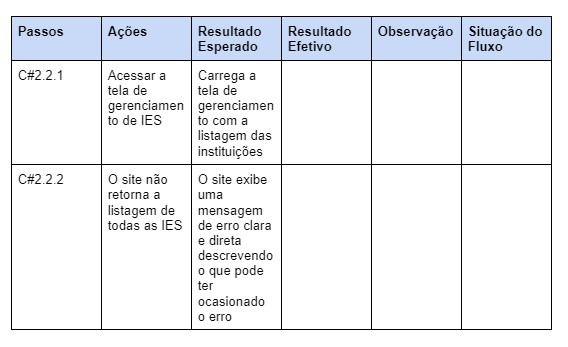
\includegraphics[width=0.80\textwidth]{images/teste-list-instituicao-excecao.jpg}
        \caption{Cenário de exceção de listagem de instituição}
        \label{commitsAturo}
    \end{figure}

O processo com exceções de listagem de instituição percorre duas ações para ser concluído.

\newpage
     
     \item \textbf{Cenário Ideal Detalhamento de instituição:}
Descrição do cenário ideal de usabilidade do usuário no processo de detalhamento de instituição.

\begin{figure}[ht]
        \centering
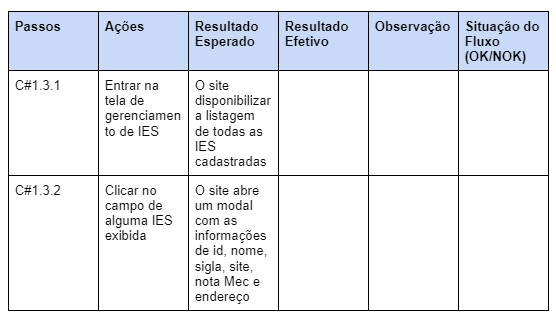
\includegraphics[width=0.80\textwidth]{images/teste-det-instituicao-feliz.jpg}
        \caption{Cenário ideal de detalhamento de instituição}
        \label{commitsAturo}
    \end{figure}

O processo ideal de detalhamento de instituição percorre duas ações para ser concluído.

\newpage

     \item \textbf{Cenário de Exceção Detalhamento de instituição:}
Descrição do cenário de exceções de usabilidade do usuário no processo de detalhamento de instituição.

\begin{figure}[ht]
        \centering
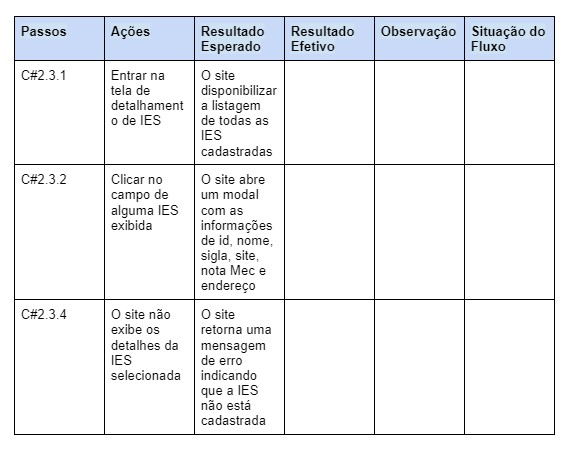
\includegraphics[width=1.0\textwidth]{images/teste-det-instituicao-excecao.jpg}
        \caption{Cenário de exceção de detalhamento de instituição}
        \label{commitsAturo}
    \end{figure}

O processo com exceções de detalhamento de instituição percorre três ações para ser concluído.

\newpage
     
     \item \textbf{Cenário Ideal Associação de Instituição com Curso:}
Descrição do cenário ideal de usabilidade do usuário no processo de associação de instituição com curso.

\begin{figure}[ht]
        \centering
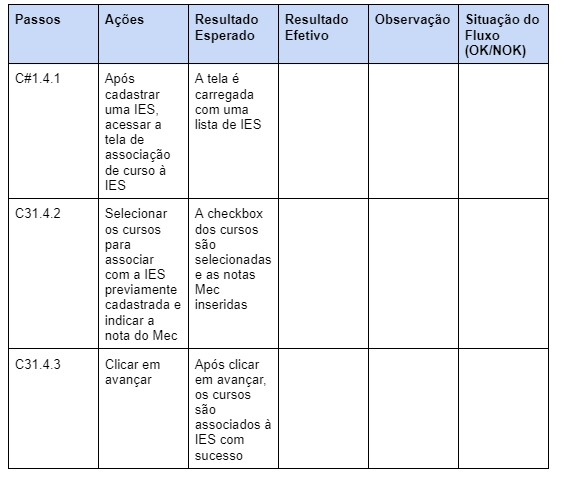
\includegraphics[width=1.0\textwidth]{images/teste-asso-instituicao-curso-feliz.jpg}
        \caption{Cenário ideal de associação de instituição com curso}
        \label{commitsAturo}
    \end{figure}

O processo ideal de associação de instituição com curso percorre três ações para ser concluído.


\newpage

\item \textbf{Cenário de Exceção Associação de Instituição com Curso:}
Descrição do cenário de exceções de usabilidade do usuário no processo de associação de instituição com curso.

\begin{figure}[ht]
        \centering
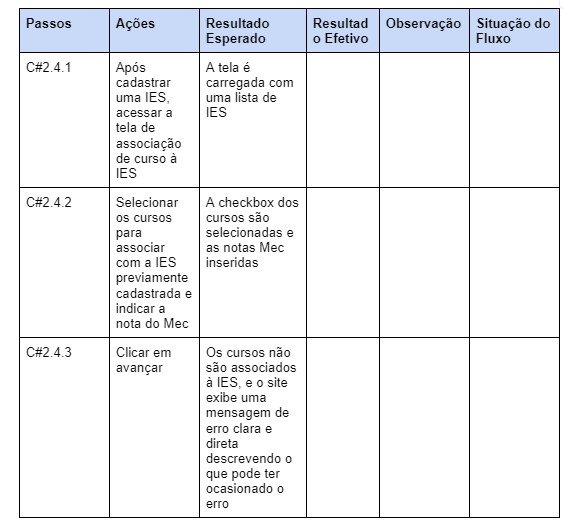
\includegraphics[width=1.0\textwidth]{images/teste-asso-instituicao-curso-excecao.jpg}
        \caption{Cenário de exceção associação de instituição com curso}
        \label{commitsAturo}
    \end{figure}

O processo com exceções de associação de instituição com curso percorre três ações para ser concluído.


\newpage

    \item \textbf{Cenário Ideal Exclusão de Instituição:}
Descrição do cenário ideal de usabilidade do usuário no processo de exclusão de instituição.


\begin{figure}[ht]
        \centering
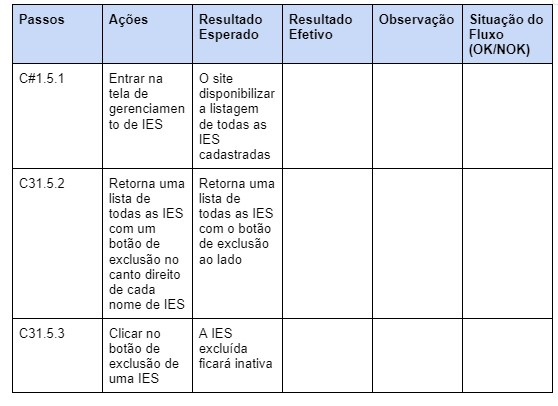
\includegraphics[width=1.0\textwidth]{images/teste-exc-instituicao-feliz.jpg}
        \caption{Cenário ideal de exclusão de instituição}
        \label{commitsAturo}
    \end{figure}

O processo ideal de exclusão de instituição percorre três ações para ser concluído.

\newpage

 \item \textbf{Cenário de Exceção Exclusão de Instituição:}
Descrição do cenário de exceções de usabilidade do usuário no processo de exclusão de instituição.

\begin{figure}[ht]
        \centering
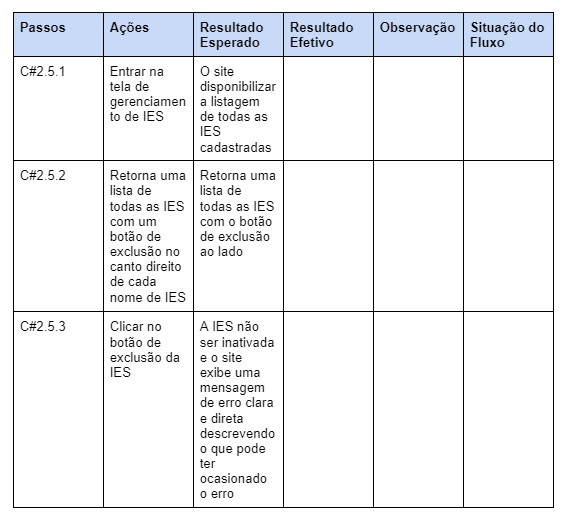
\includegraphics[width=0.75\textwidth]{images/teste-exc-instituicao-excecao.jpg}
        \caption{Cenário de exceção de exclusão de instituição}
        \label{commitsAturo}
\end{figure}
O processo com exceções de exclusão de instituição com curso percorre três ações para ser concluído.

\end{itemize}

A partir dos cenários de teste apresentados, torna-se viável simular um eventual caminho alternativo que o usuário final pode enfrentar durante a sua experiência navegando pelo site. Dessa forma, é possível realizar uma análise voltada à visão do usuário final, buscando suprir suas necessidades e melhorar a usabilidade do site.



